\documentclass{article} 
\usepackage{neurips_2025}
\usepackage[utf8]{inputenc}
\usepackage[vietnamese]{babel} 
\usepackage[T1]{fontenc}
\usepackage{hyperref}
\usepackage{url}
\usepackage{booktabs}
\usepackage{amsfonts}
\usepackage{amsmath}
\usepackage{microtype}
\usepackage{xcolor}
\usepackage{graphicx}
\usepackage{float}
\usepackage{enumitem}
\usepackage{mdframed}
\usepackage{tabularx}
\usepackage{multicol} 
\usepackage{graphicx}
\usepackage{float}
\usepackage{subcaption}
\usepackage[strings]{underscore}
\usepackage[justification=centering]{caption}

\setlength{\parskip}{3pt} 
\setlength{\parindent}{12pt}
\setlength{\columnsep}{18pt}

\newmdenv[
  backgroundcolor=gray!06,
  linecolor=gray!25,
  linewidth=0.5pt, 
  innerleftmargin=5pt, 
  innerrightmargin=5pt,
  innertopmargin=5pt, 
  innerbottommargin=5pt, 
  skipabove=8pt, 
  skipbelow=8pt,
  leftmargin=0pt, 
  rightmargin=0pt
]{phbox}

\newcommand{\figbox}[2][90pt]{%
  \begin{center}
    \fbox{\parbox{0.96\linewidth}{\centering\rule{0pt}{#1}%
    \small\textit{#2}}}
  \end{center}
}

\definecolor{gridgreen}{RGB}{34, 115, 48} 

\title{
    \huge \textcolor{gridgreen}{\textbf{DATATHON 2026}} \\
    \vspace{4pt}
    \Large {Tối ưu hóa vận hành E-Commerce: \\Phân tích Hành vi Khách hàng và Hệ Thống Dự báo Doanh thu} \\
}

\author{
  \textbf{Đội Data Manipulators} \\
  \vspace{8pt} \\
  \begin{minipage}[t]{0.31\textwidth}
    \centering
    \small \textbf{Đỗ Mai Hằng} \\
    \scriptsize ĐH Công nghệ - ĐHQGHN \\ 
    \scriptsize (Hệ thống thông tin) \\
    \texttt{24022647@vnu.edu.vn} \\
  \end{minipage}
  \hfill
  \begin{minipage}[t]{0.31\textwidth}
    \centering
    \small \textbf{Khoa Đào Ngọc Bích} \\
    \scriptsize ĐH Công nghệ - ĐHQGHN \\ 
    \scriptsize (Khoa học máy tính) \\
    \texttt{24021388@vnu.edu.vn} \\
  \end{minipage}
  \hfill
  \begin{minipage}[t]{0.31\textwidth}
    \centering
    \small \textbf{Từ Thị Thu Uyên} \\
    \scriptsize Học viện Tài chính \\ 
    \scriptsize (Hệ thống thông tin quản lý) \\
    \texttt{tuthithuuyen.0105@hvtc.edu.vn} \\
  \end{minipage}
  \and
  \vspace{8pt} \\
  \small\texttt{\url{https://github.com/Jade2612/DATATHON}}
}

\begin{document}

\maketitle

\begin{abstract}
\small
Dự báo nhu cầu chính xác là yếu tố then chốt để tối ưu hóa tồn kho và logistics cho doanh nghiệp thương mại điện tử thời trang tại Việt Nam. Báo cáo này kết hợp phân tích chuyên sâu (EDA) để khám phá hành vi mua sắm đặc thù trong các kỳ Tết và Mega-sale với hệ thống dự báo sử dụng \textbf{Ensemble LightGBM, XGBoost và N-HiTS}. Bằng cách khai thác hơn 70 đặc trưng sáng tạo như độ trễ lưu lượng web và chỉ số khuyến mãi, mô hình đạt độ chính xác cao với điểm Kaggle đạt 933412,90305. Kết quả không chỉ cung cấp con số dự báo mà còn là câu chuyện về dữ liệu, giúp doanh nghiệp chủ động lập kế hoạch logistics và khuyến mãi hiệu quả trên toàn quốc.
\end{abstract}

\vspace{5pt}
\hrule
\vspace{12pt}

\begin{multicols}{2}

\section{Giới thiệu}

\section{Trực quan hoá và Phân tích EDA}

\subsection{Vấn đề trả hàng không đến từ chất lượng sản phẩm mà là sizing}


Tổng số đơn return khoảng 25.800 đơn và 109.000 sản phẩm với doanh thu mất từ các đơn này là 650M đồng(4.15\% tổng doanh thu). Trong đó danh mục streetwear là danh mục bị trả về nhiều nhất, ảnh hưởng đáng kể đến doanh thu, với 21799 đơn return đã gây ra tổn thất đến 474.9M đồng(79,9\% tổng tổn thất) với size bị trả về nhiều nhất là XL với 16,7\%. Wrong size chiếm khoảng 35\% cho hầu như đồng đều các danh mục sản phẩm và đây là lí do trả về chiếm tỉ trọng cao nhất, cứ 100 đơn đặt hàng thì 1.2-1.3 đơn bị hoàn vì wrong size tùy danh mục. Vấn đề wrong size cũng là tình trạng chung xảy ra ở hầu hết các thành phố, từ những điều này cho thấy vấn đề không xuất phát từ một nhóm sản phẩm cụ thể hay một khu vực cụ thể mà là một vấn đề mang tính hệ thống, có thể do nhiều nguyên nhân như size guide chưa tốt, sản phẩm chưa đúng các thông số kĩ thuật hoặc nằm ở khách hàng chọn sai size, cần thêm data về feedback khách hàng để xác định nguyên nhân chính xác. Tỉ lệ này sẽ không cải thiện nếu không có thay đổi về trải nghiệm chọn size.

\begin{center}
    \begin{minipage}{\linewidth} 
        \centering
        \begin{subfigure}{0.31\linewidth}
            \centering
            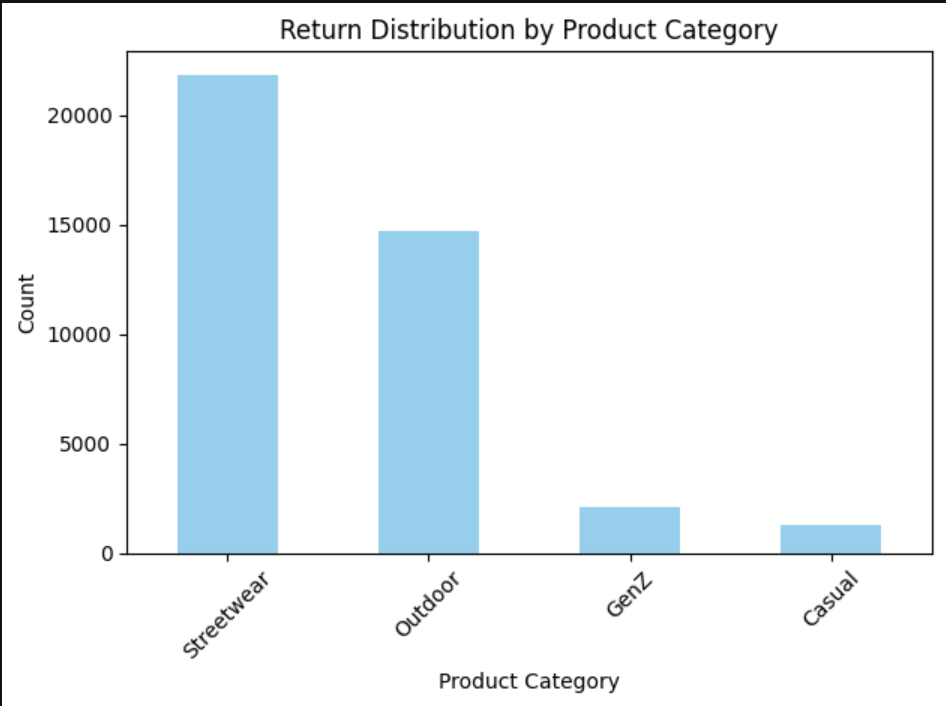
\includegraphics[width=\linewidth]{figures/return_dis_by_category.png}
            \caption{\scriptsize Chart 1}
        \end{subfigure}
        \hfill
        \begin{subfigure}{0.31\linewidth}
            \centering
            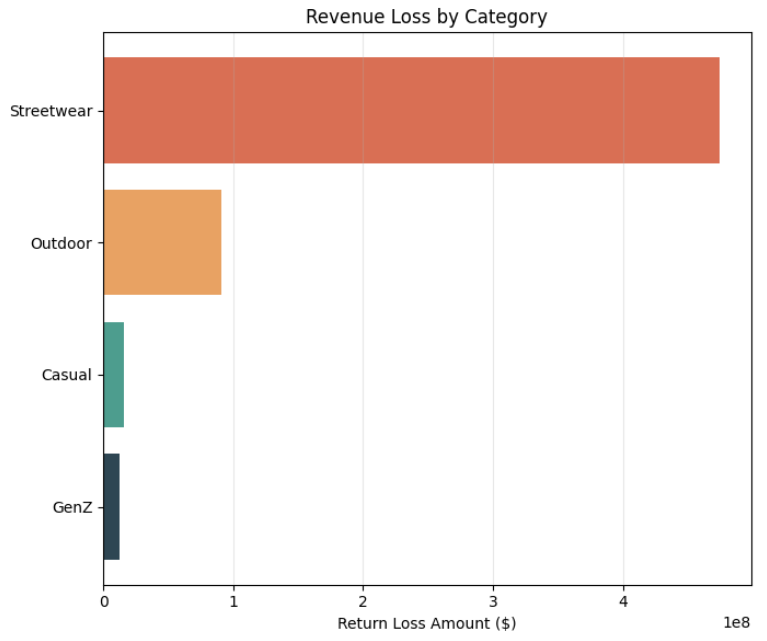
\includegraphics[width=\linewidth]{figures/revenue_loss_by_category.png}
            \caption{\scriptsize Chart 2}
        \end{subfigure}
        \hfill
        \begin{subfigure}{0.31\linewidth}
            \centering
            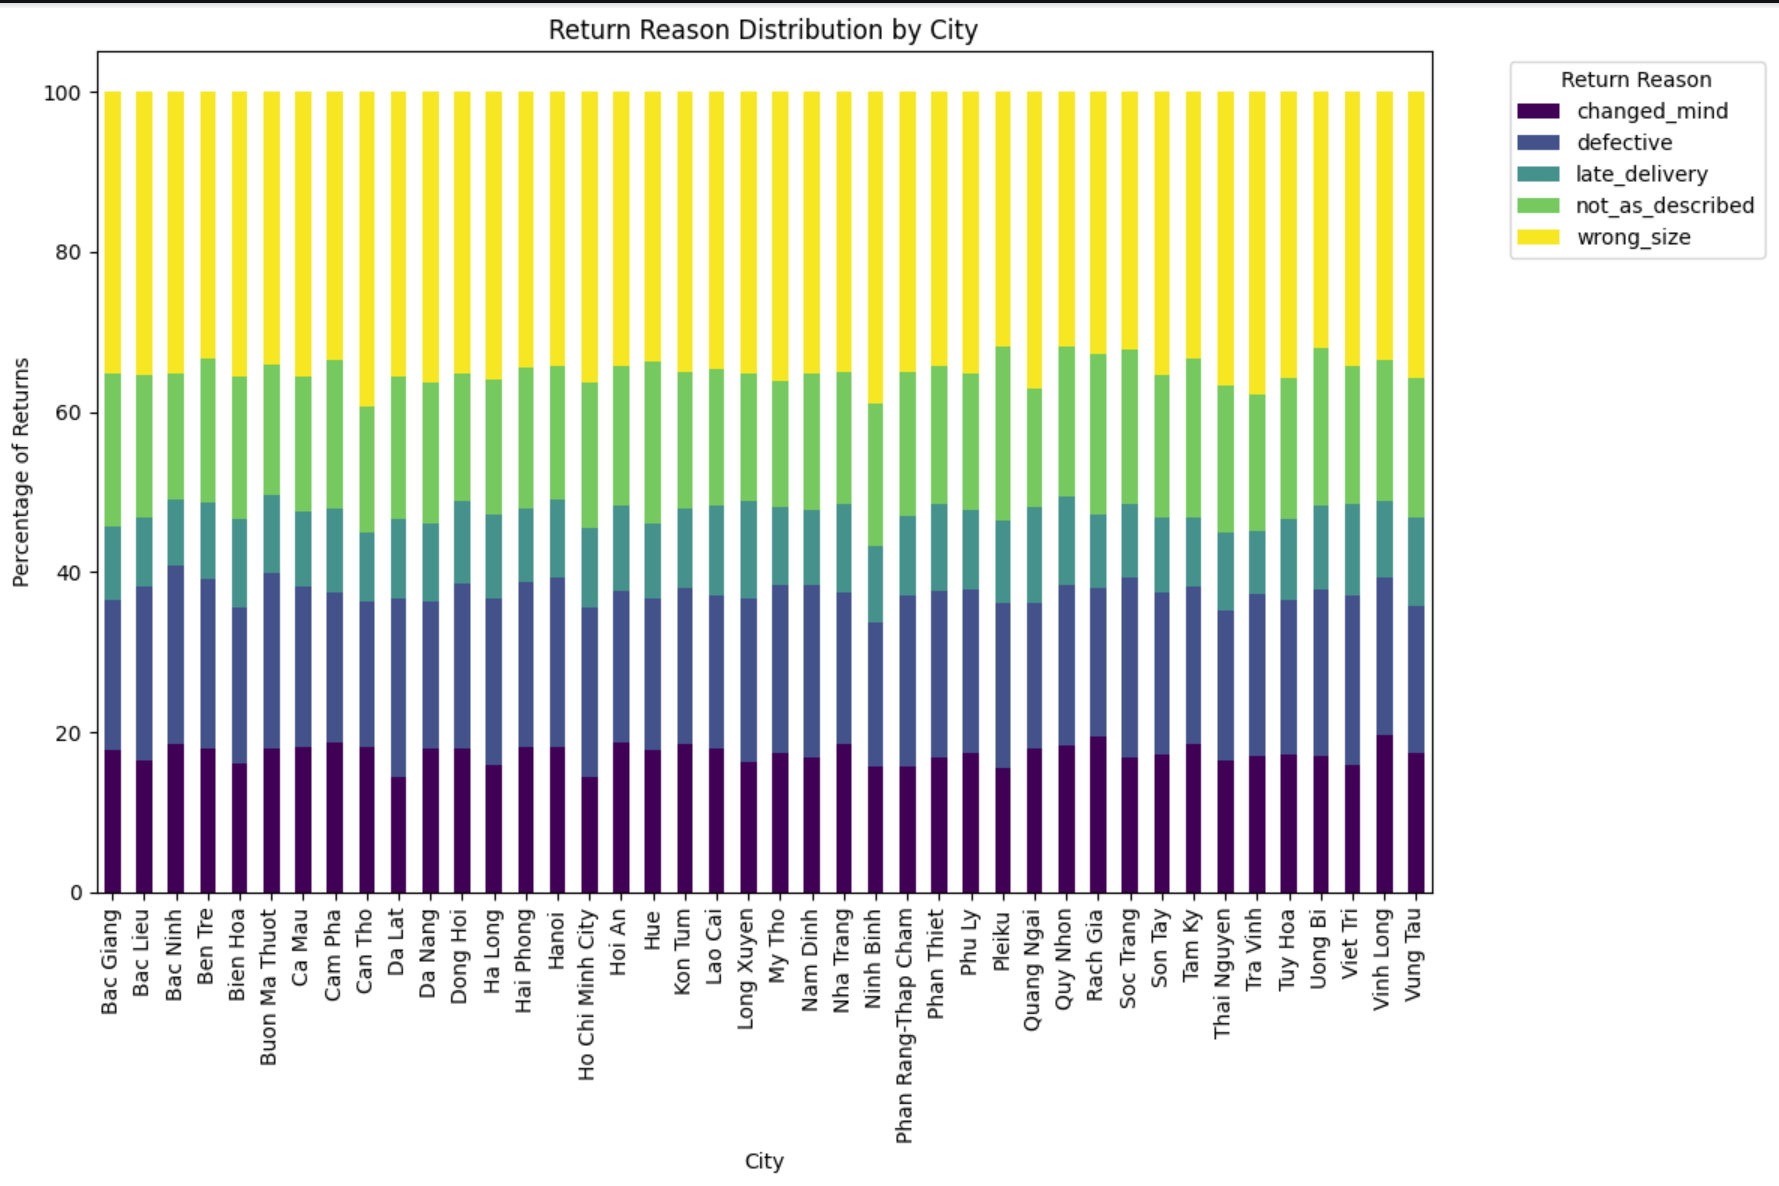
\includegraphics[width=\linewidth]{figures/return_dis_by_city.png}
            \caption{\scriptsize Chart 3}
        \end{subfigure}

        \captionof{figure}{Tỉ lệ trả hàng theo danh mục\\
        Doanh thu mất theo danh mục\\
        Tỉ lệ trả hàng theo các lí do theo thành phố}
        \label{fig:three_charts}
    \end{minipage}
\end{center}

\begin{center}
    \begin{minipage}{\linewidth} 
        \centering
        \begin{subfigure}{0.31\linewidth}
            \centering
            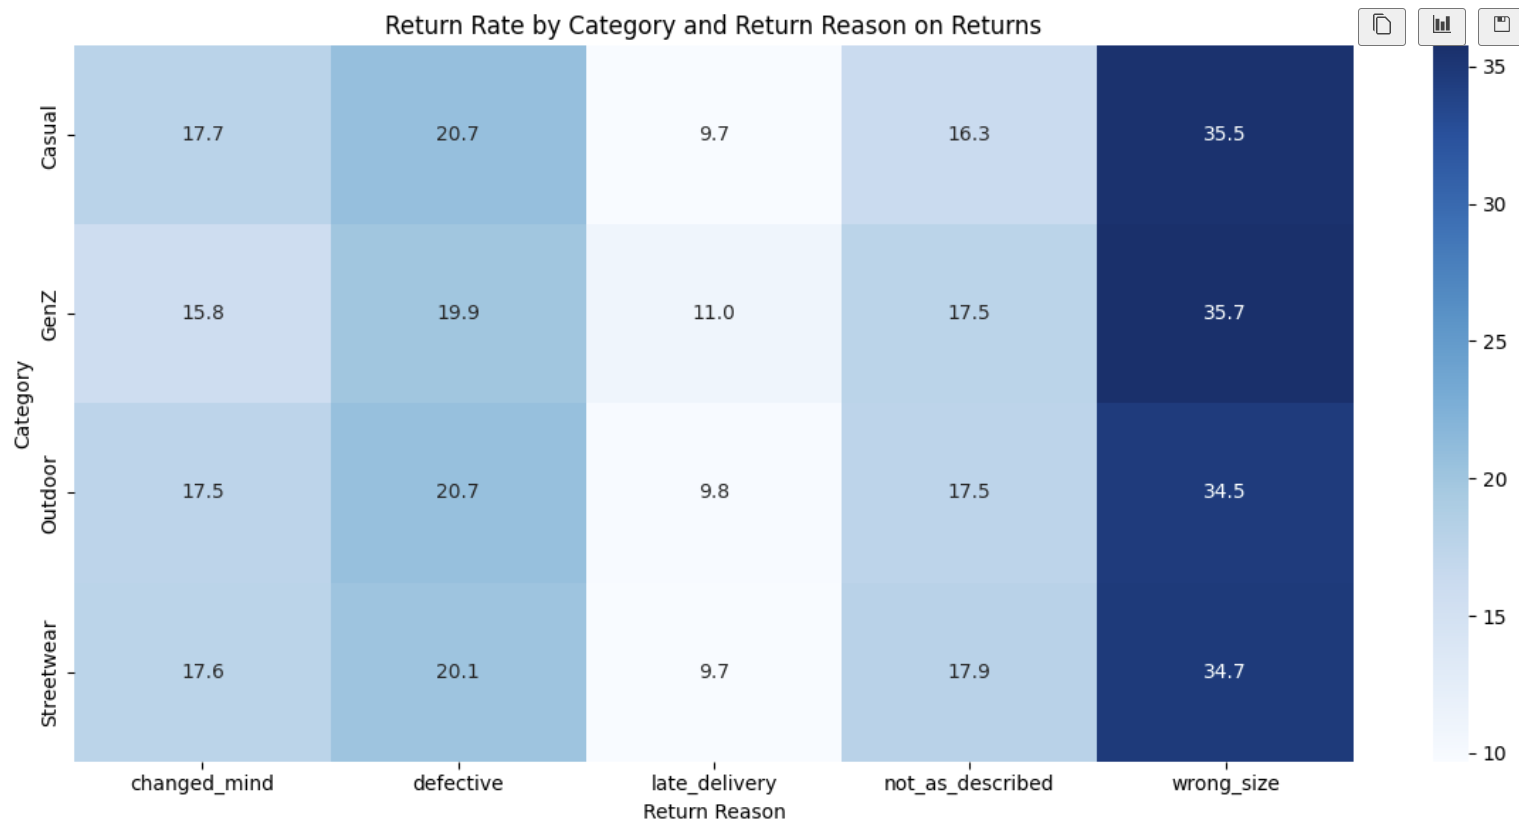
\includegraphics[width=\linewidth]{figures/return_rate_by_cate_reason_returns.png}
            \caption{\scriptsize Chart 1}
        \end{subfigure}
        \hfill
        \begin{subfigure}{0.31\linewidth}
            \centering
            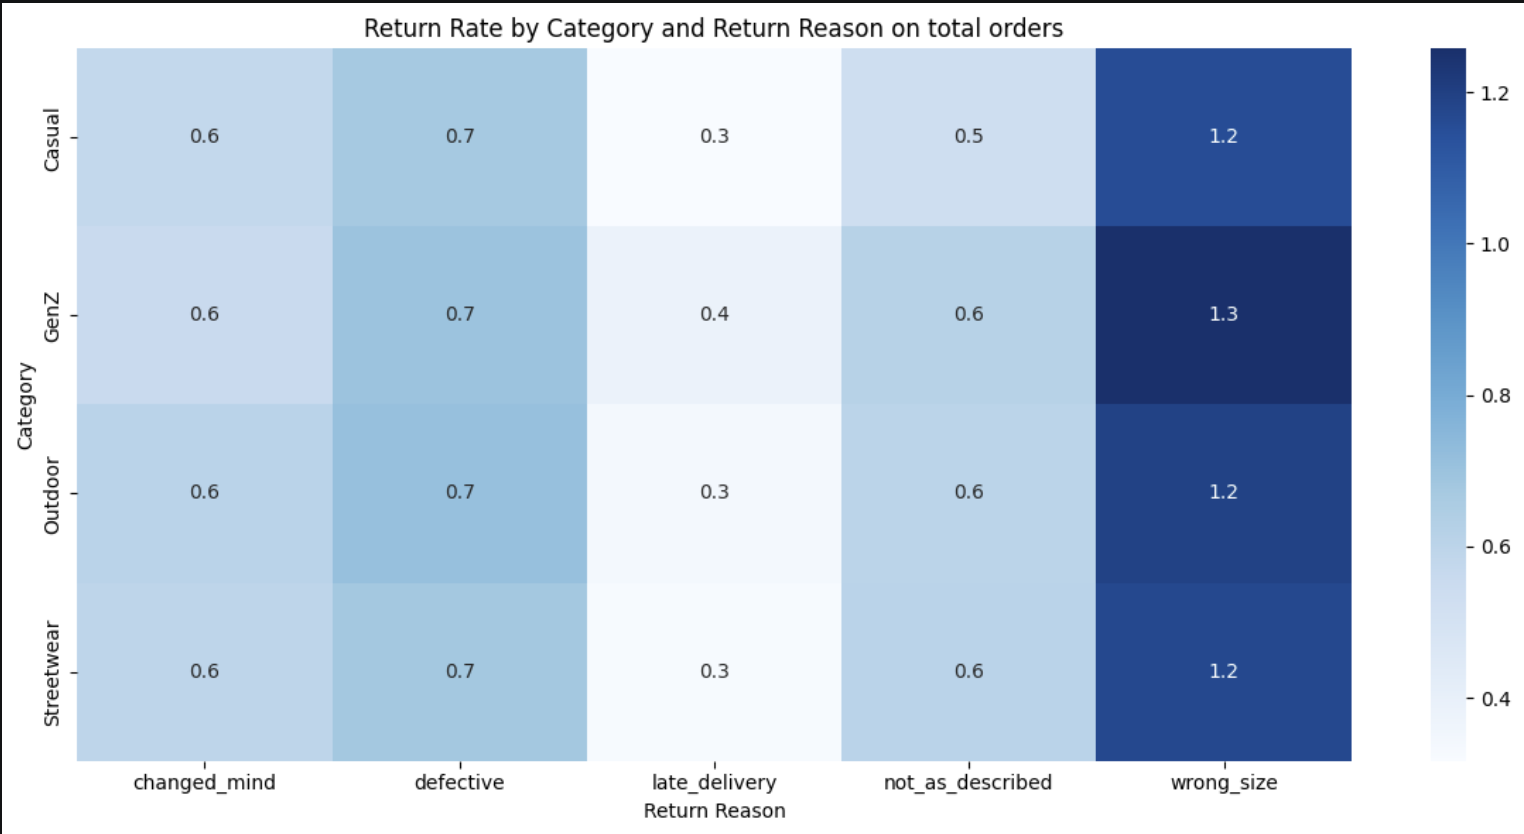
\includegraphics[width=\linewidth]{figures/return_rate_by_cate_reason_total.png}
            \caption{\scriptsize Chart 2}
        \end{subfigure}
        \hfill
        \begin{subfigure}{0.31\linewidth}
            \centering
            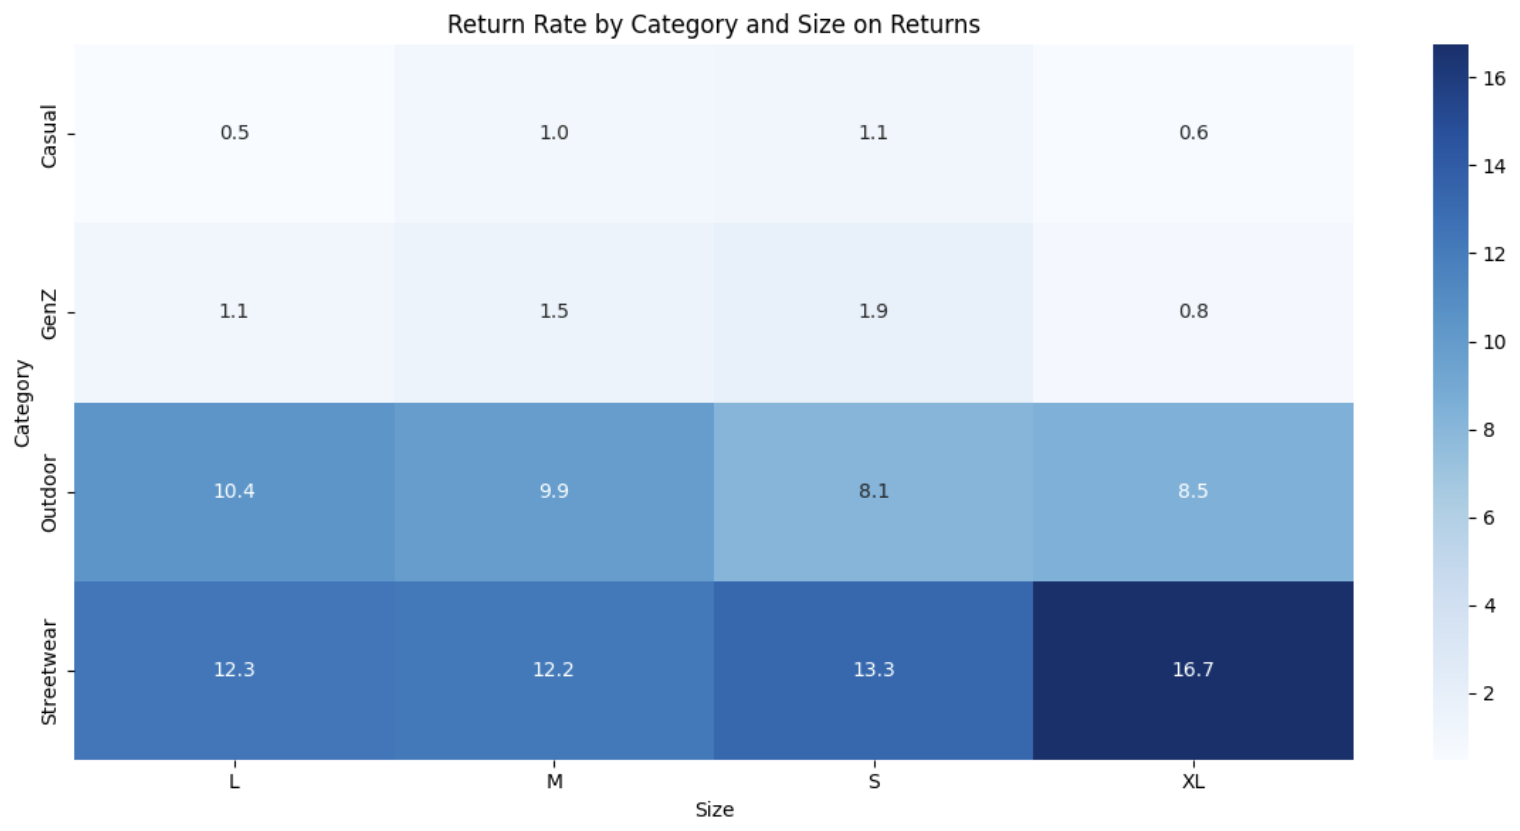
\includegraphics[width=\linewidth]{figures/return_rate_cate_size.png}
            \caption{\scriptsize Chart 3}
        \end{subfigure}

        \captionof{figure}{Tỉ lệ trả hàng theo danh mục và lí do trên các đơn hàng được hoàn trả\\
        Tỉ lệ trả hàng theo danh mục và lí do trên tổng các đơn hàng\\
        Tỉ lệ trả hàng theo danh mục và size}
        \label{fig:three_charts}
    \end{minipage}
\end{center}
→ Đề xuất giải pháp:\\
\textbf{1. Thu thập data wrong/_size feedback} \\
Chi phí: gần như 0 (thêm câu hỏi vào flow hoàn hàng) \\
Tác động trực tiếp: không giảm return ngay, nhưng mở khóa toàn bộ Diagnostic → là tiền đề cho mọi giải pháp tiếp theo\\
Dự kiến tác động: có kết quả sau 1–2 tháng thu thập \\
\textbf{2. Cải thiện sizing experience, ưu tiên streetwear vì đây là mặt hàng gây tổn thất lớn} \\
Cơ sở: wrong size ~35/% của 650M tổn thất = ~227M liên quan wrong_size \\ 
Tác động trực tiếp: Mỗi 10/% giảm wrong size = tiết kiệm ~23M - mức giảm thực tế dựa vào nguyên nhân gốc rễ xác định được từ feedback data\\
Cách triển khai: bảng size chi tiết theo số đo các vòng cụ thể, size guide riêng theo danh mục, có ảnh mẫu mặc với ghi chú chiều cao cân nặng giúp người dùng hình dung rõ nhất về size sản phẩm thay vì chỉ chọn dựa vào ảnh \\
\textbf{3. Đổi size miễn phí hoặc có phí trong giới hạn ngày nhất định từ khi nhận hàng } \\
Tác động trực tiếp: Không giảm return rate nhưng giữ lại doanh thu và có khả năng giữ chân khách hàng dài hạn 

\subsection{}

\section{Mô hình Dự báo Doanh Thu}

\subsection{Đánh giá Hiệu suất Mô hình}

Mô hình kết hợp (Final Blend) đạt hiệu suất dự báo xuất sắc trên tập kiểm thử, giảm gần 80\% sai số so với mô hình cơ sở (Baseline). Với $R^2 = 0.9573$, mô hình giải thích được hơn 95\% sự biến thiên của doanh thu thực tế. Các chỉ số sai số (MAE, RMSE) được kiểm soát ở mức rất thấp cung cấp một công cụ hoạch định ngân sách và chuỗi cung ứng với độ tin cậy cao, giúp doanh nghiệp chủ động giảm thiểu rủi ro tồn kho.

\begin{center}
\small
\textbf{Bảng 1: Đánh giá hiệu suất tổng thể (MAE)} \\
\vspace{0.1cm}
\begin{tabularx}{\linewidth}{lXX}
\toprule
\textbf{Mô hình} & \textbf{Doanh thu} & \textbf{COGS} \\
\midrule
Baseline & 1,181,818 & 915,396 \\
N-HiTS & 2,000,078 & - \\
LightGBM & 757,238 & 659,777 \\
\textbf{Final Blend} & \textbf{242,978} & \textbf{659,777} \\
\bottomrule
\end{tabularx}
\end{center}
\textbf{Kaggle score:} 933412,90305\\
\textit{
\textbf{Đối với Doanh thu:} LightGBM /(67.2/%) và XGBoost (32.8/%). Trọng số của N-HiTS tự động bị ép về 0\% do sai số lớn. \\
\textbf{Đối với COGS:} Thuật toán tối ưu tự động lựa chọn 100/% trọng số cho LightGBM (không sử dụng XGBoost và N-HiTS).
}

\subsection{Thiết kế Hệ thống và Chất lượng Pipeline}

Toàn bộ quy trình phân tích và huấn luyện tuân thủ tuyệt đối các quy tắc và đảm bảo tính tái lập bằng việc cố định random\_seed = 42 và cung cấp mã nguồn đính kèm.

\begin{enumerate}[leftmargin=2em]
    \item \textbf{Feature Engineering}: Tạo 85 đặc trưng cốt lõi bao quát tính mùa vụ (chu kỳ Fourier, sự kiện), độ trễ (lag) và trung bình trượt (rolling/EWM).
    \item \textbf{Cross-validation}: Áp dụng Walk-forward CV (5-fold) bám sát luồng dữ liệu thời gian thực, đánh giá chính xác năng lực dự báo và tránh overfitting.
    \item \textbf{Xử lý Leakage}: Dùng cơ chế dự báo đệ quy (Recursive Forecasting) cập nhật liên tục các biến trễ, triệt tiêu hoàn toàn hiện tượng rò rỉ dữ liệu.
\end{enumerate}

\subsection{SHAP và Feature Importance}
\begin{figure}[H]
    \centering
    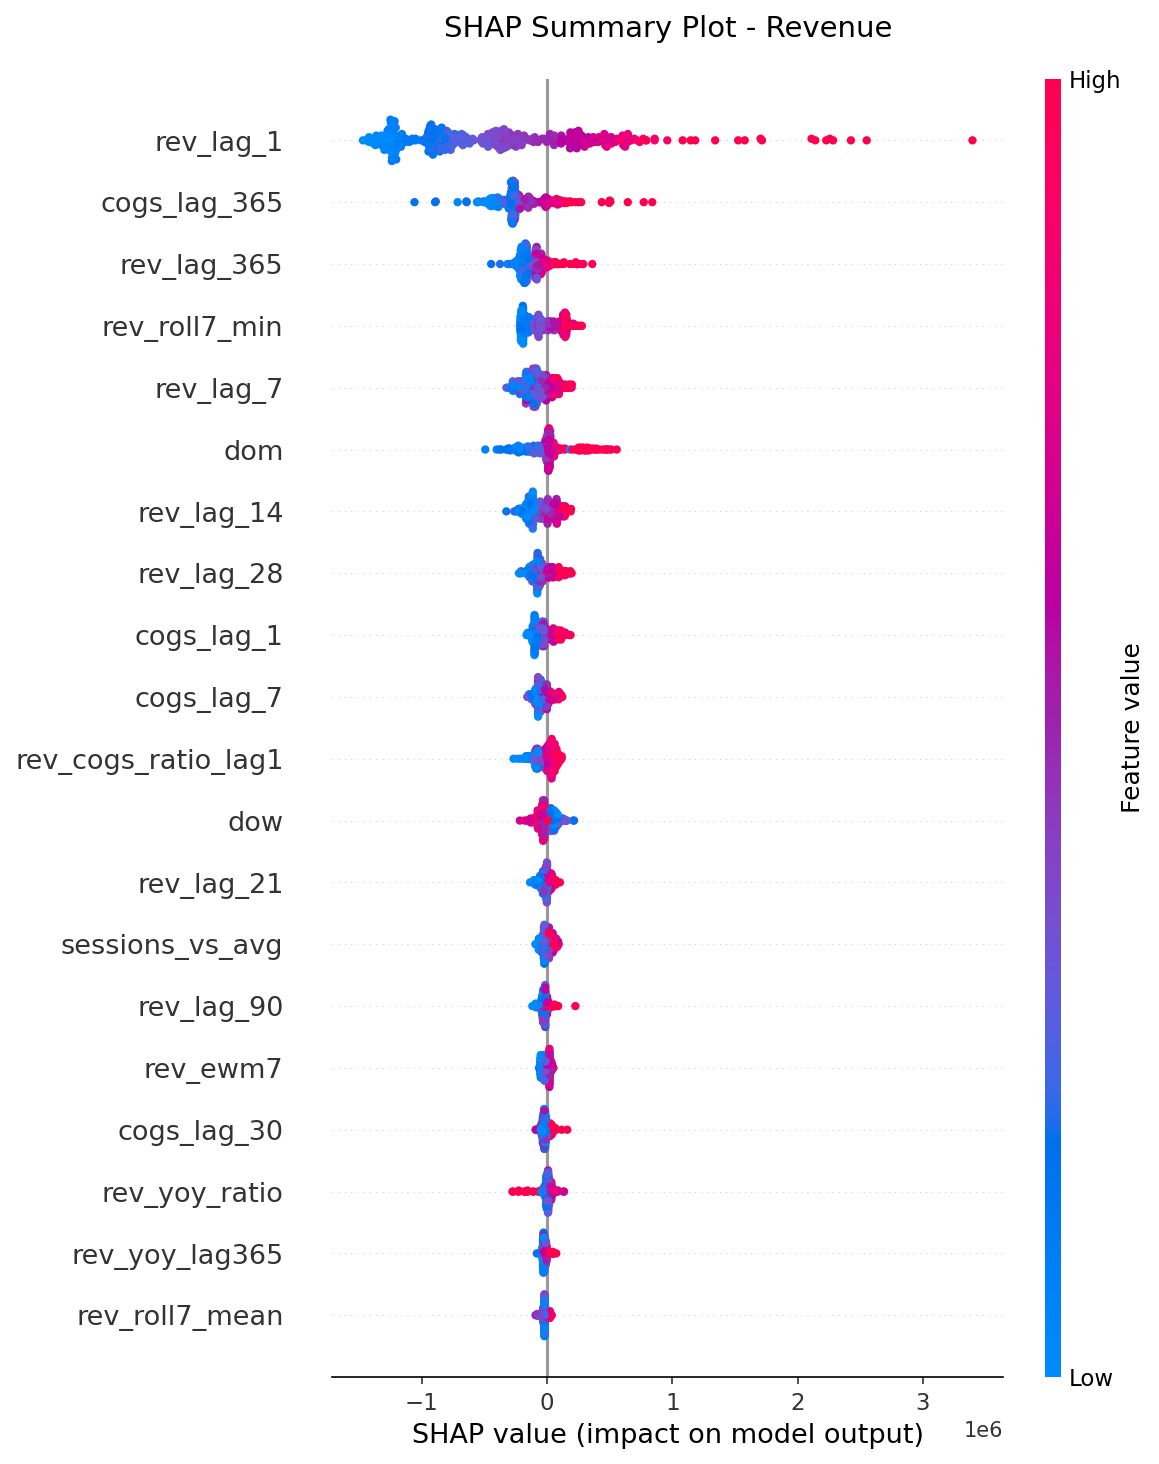
\includegraphics[width=0.8\linewidth]{figures/shap_summary.png}
    \caption{Biểu đồ SHAP Feature Importance cho mô hình Ensemble dự báo Doanh thu.}
    \label{fig:revenue_2022}
\end{figure}

\begin{figure}[H]
    \centering
    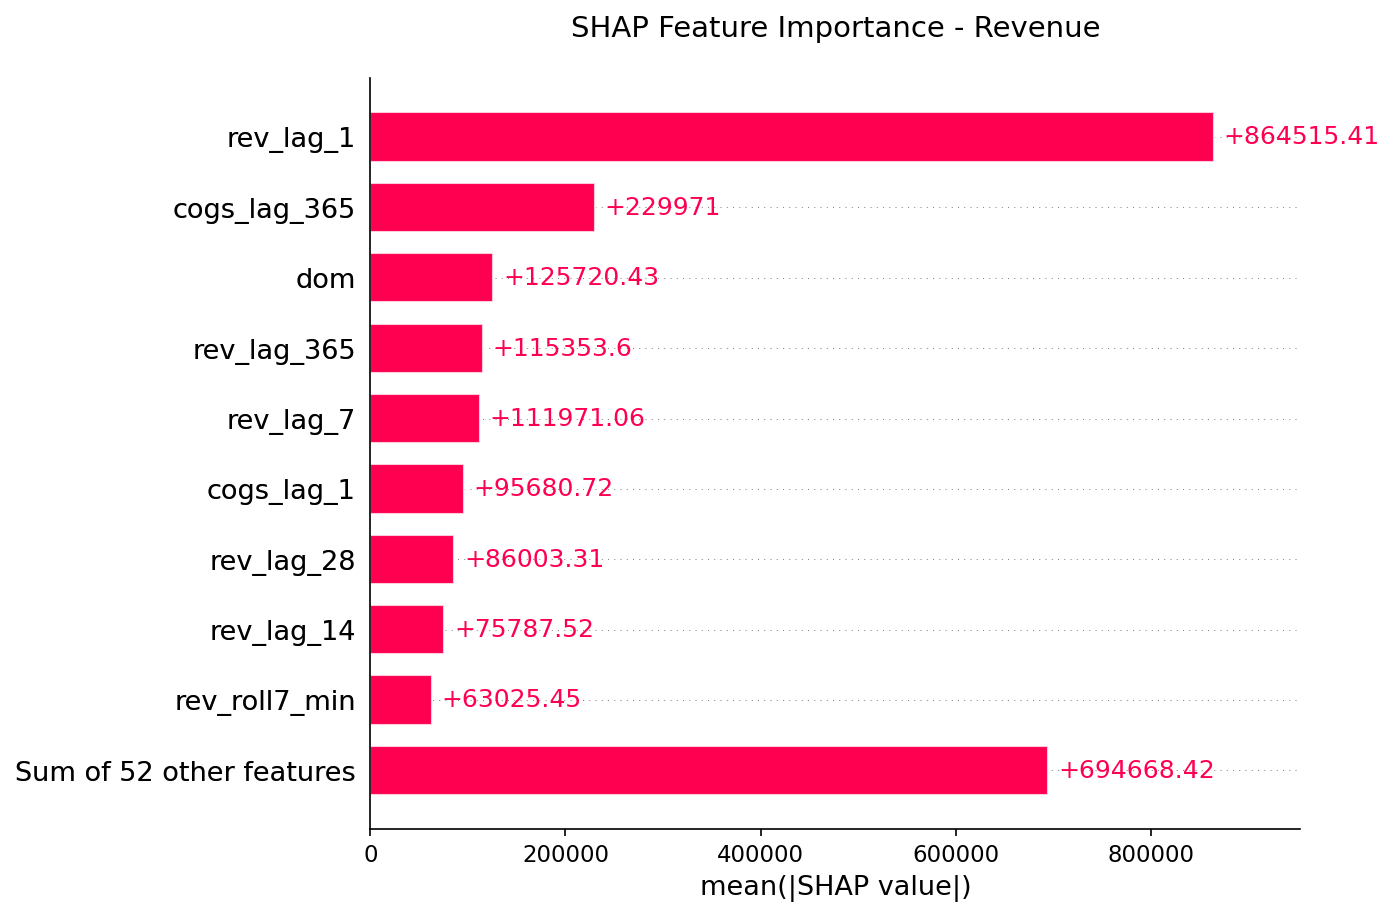
\includegraphics[width=0.8\linewidth]{figures/feature_importance.png}
    \caption{Top features theo mean $|\mathrm{SHAP}|$}
    \label{fig:revenue_2022}
\end{figure}
Thông qua phân tích SHAP Summary và Feature Importance, mô hình đã chỉ ra 3 nhóm yếu tố cốt lõi thực sự quyết định doanh thu của doanh nghiệp:
\begin{enumerate}[leftmargin=2em]
    \item \textbf{Đà mua sắm ngắn hạn \& Chu kỳ tuần}: Các biến độ trễ gần (\texttt{rev\_lag\_1}, \texttt{cogs\_lag\_1}) và chu kỳ tuần (\texttt{lag\_7, 14, 28}) chi phối mạnh nhất, phản ánh đà chi tiêu tiếp nối của khách hàng từ những ngày trước.
    \item \textbf{Tham chiếu lịch sử (Cùng kỳ năm ngoái)}: Dữ liệu trễ đúng 1 năm (\texttt{cogs\_lag\_365}, \texttt{rev\_lag\_365}) lọt top đầu, đóng vai trò là "mỏ neo" cơ sở để hiệu chỉnh doanh thu năm nay.
    \item \textbf{Thói quen định kỳ \& Chu kỳ vĩ mô}: Ngày trong tháng (\texttt{dom}) và sóng Fourier (\texttt{fourier\_sin\_p365\_25\_k1}) nắm bắt cực tốt các hành vi lặp lại (như kỳ nhận lương) và dòng chảy mùa vụ tổng thể.
\end{enumerate}
Chúng ta có thể nhìn rõ hơn thông qua 2 biểu đồ dưới đây:
\begin{figure}[H]
    \centering
    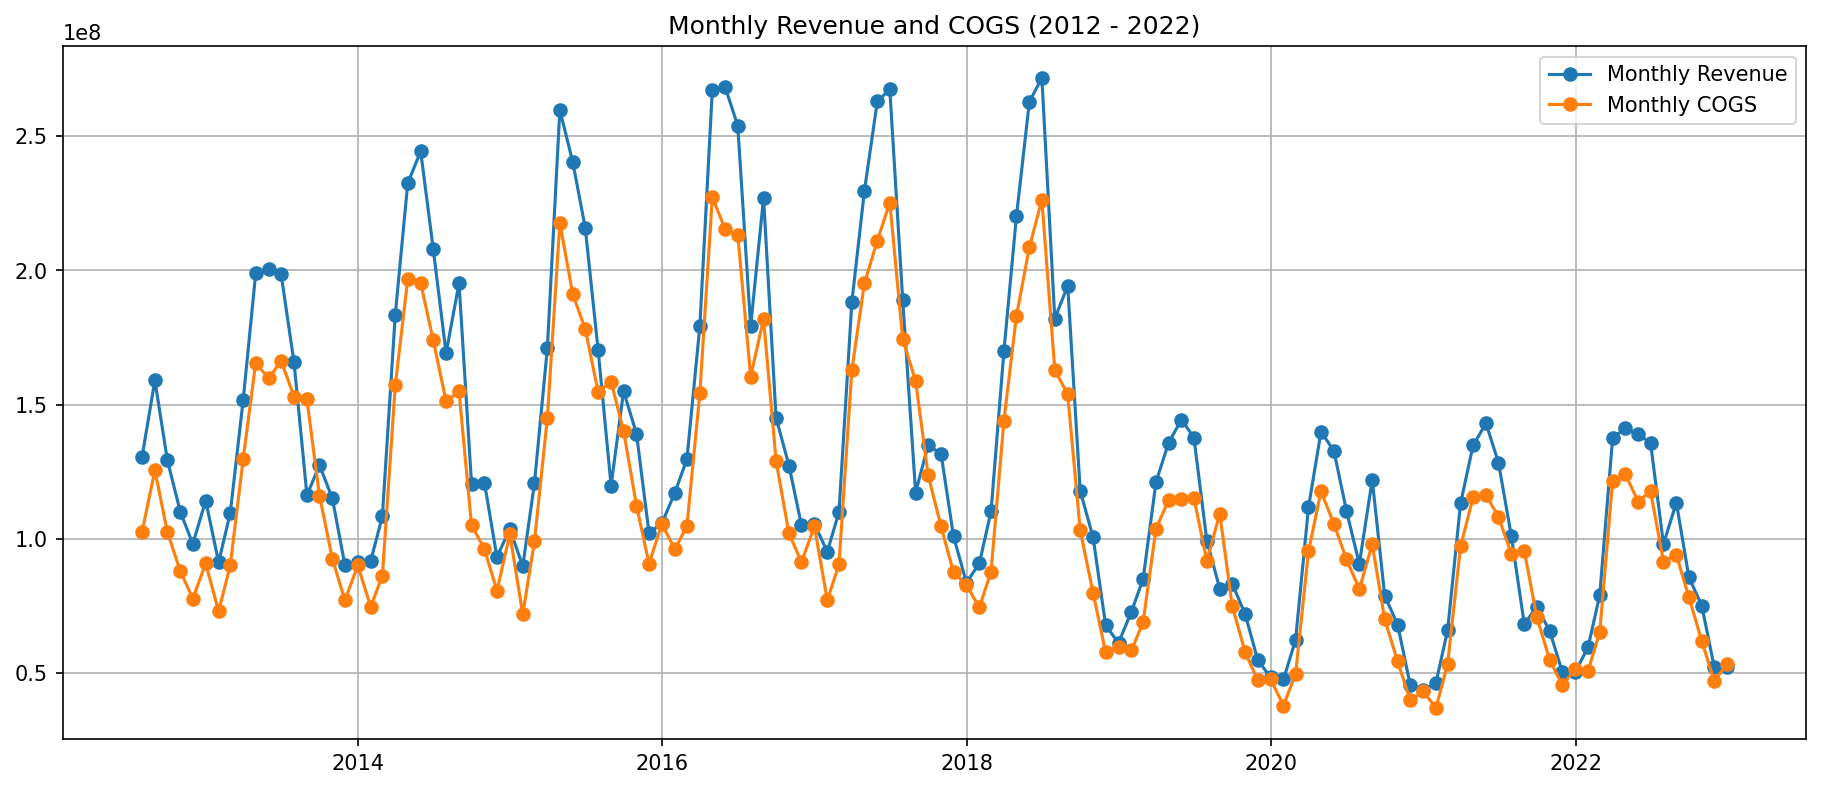
\includegraphics[width=0.8\linewidth]{figures/monthly_revenue_and_cogs.png}
    \caption{Diễn biến doanh thu và giá vốn hàng bán (COGS) theo tháng}
    \label{fig:revenue_cogs}
\end{figure}
\begin{figure}[H]
    \centering
    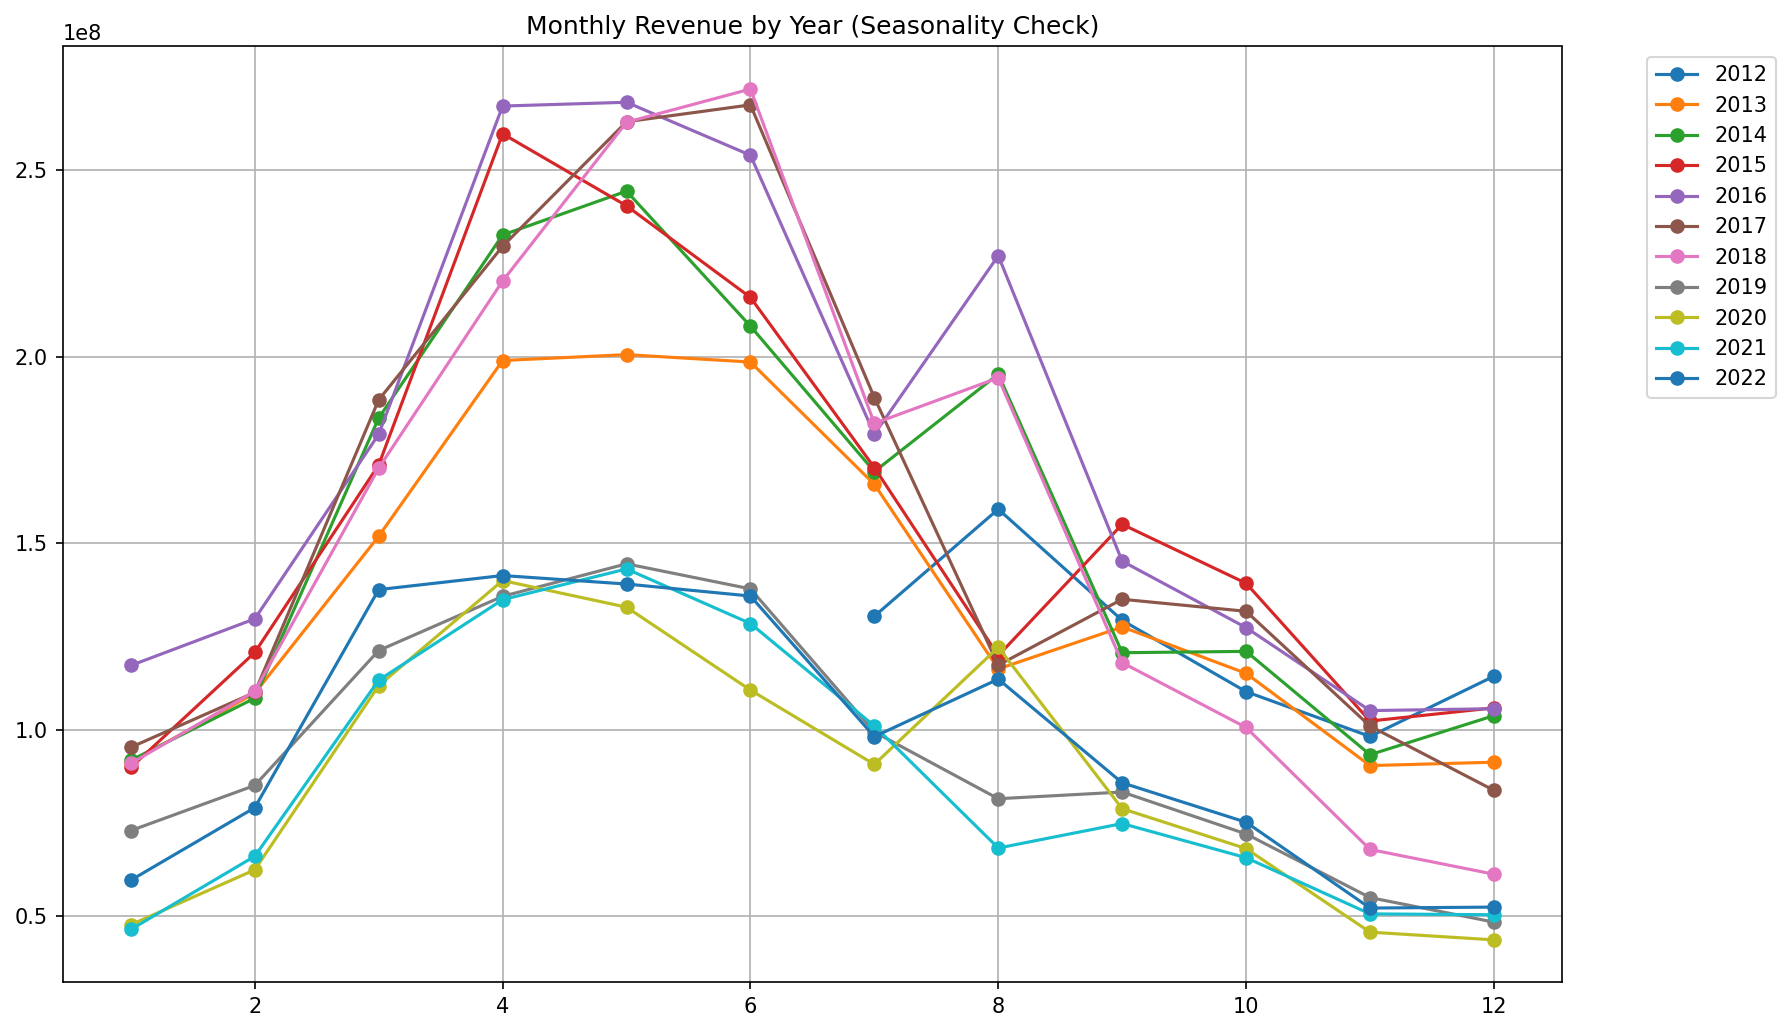
\includegraphics[width=0.8\linewidth]{figures/monthly_revenue_by_year.png}
    \caption{So sánh doanh thu hàng tháng giữa các năm}
    \label{fig:revenue_year}
\end{figure}

\section{Mã nguồn}
\url{https://github.com/Jade2612/DATATHON}

\begingroup
\scriptsize 
\setlength{\itemsep}{0pt} 
\nocite{*}
\bibliographystyle{unsrt} 
\bibliography{references} 
\endgroup

\end{multicols}
\end{document}